\documentclass[a4paper, 11pt]{report}
\usepackage[margin=1in]{geometry}
\usepackage{listings}
\usepackage[strings]{underscore}
\usepackage{dirtytalk}
\usepackage{xcolor}
\usepackage{multicol}
\usepackage{multirow}
\usepackage{graphicx}
\usepackage{pdfpages}
\usepackage{appendix}
\usepackage{float}
\usepackage{booktabs}
\usepackage{hyperref}
\usepackage[acronym,toc]{glossaries}

\definecolor{comment}{RGB}{0,128,0} % dark green
\definecolor{string}{RGB}{255,0,0}  % red
\definecolor{keyword}{RGB}{0,0,255} % blue
\graphicspath{ {./images/} }

\loadglsentries{glossary}
\makeglossaries

\lstdefinestyle{c}{
	commentstyle=\color{comment},
	stringstyle=\color{string},
	keywordstyle=\color{keyword},
	basicstyle=\footnotesize\ttfamily,
	numbers=left,
	numberstyle=\tiny,
	numbersep=5pt,
	frame=lines,
	breaklines=true,
	prebreak=\raisebox{0ex}[0ex][0ex]{\ensuremath{\hookleftarrow}},
	showstringspaces=false,
	upquote=true,
	tabsize=2,
}

\lstdefinestyle{java}{
	commentstyle=\color{comment},
	stringstyle=\color{string},
	keywordstyle=\color{keyword},
	basicstyle=\footnotesize\ttfamily,
	numbers=left,
	numberstyle=\tiny,
	numbersep=5pt,
	frame=lines,
	breaklines=true,
	prebreak=\raisebox{0ex}[0ex][0ex]{\ensuremath{\hookleftarrow}},
	showstringspaces=false,
	upquote=true,
	tabsize=2,
}

%%%%%%%%%%%%%%%%%%
% TITLE
%%%%%%%%%%%%%%%%%%
\title{\Huge{\textbf{Using Blockchain to Create a Decentralised Security Model for Distributed Systems}}}
\date{April 2021}
\author{\Large{Adam David Bruce} \\ \texttt{\href{mailto:a.bruce3@newcastle.ac.uk}{a.bruce3@newcastle.ac.uk}}}
\begin{document}
\maketitle

%%%%%%%%%%%%%%%%%%
% ABSTRACT
%%%%%%%%%%%%%%%%%%
\begin{abstract}
//TODO
\end{abstract}

%%%%%%%%%%%%%%%%%%
% TABLE OF CONTENTS, FIGURES and TABLES
%%%%%%%%%%%%%%%%%%
\tableofcontents
\listoffigures
\listoftables

\newpage

%%%%%%%%%%%%%%%%%%
% INTRODUCTION
%%%%%%%%%%%%%%%%%%
\chapter{Introduction}
\section{COVID-19 and Cyberattacks}
In the summer of 2020 during the midst of the COVID-19 pandemic, universities and research institutions worldwide were working hard to understand the structure of the virus and develop a vaccine in an attempt to return to normality. However, whereas some countries were making fast progress in understanding the virus, others were falling behind, and the virus began to put a strain on healthcare, and increasing critique on governments. In order to keep up with the nations at the forefront of vaccine development, nations turned to state-sponsored cyberattacks in order to both hinder nations, and also obtain research and information about other countries' vaccine efforts. One such example was the threat group 'Cozy Bear', formally known as \acrfull{APT} 29. \acrshort{APT}29 used a number of tools to target various organisations involved in COVID-19 vaccine development in Canada, the United States and the United Kingdom. The \acrfull{NCSC} believe that the intention was highly likely stealing information and intellectual property relating to the vaccine \cite{APT29}.

In addition to the mortality of COVID-19, the virus also caused a number of economic issues across a number of nations. Global stock markets lost \$6 trillion in value over size days from 23 to 28 February \cite{covspill}. This gave private companies no other choice than to make large volumes of staff redundant, which increased job insecurity causing many people to become redundant, and in nations without suitable support or benefits, attackers turned to cybercrime for financial gain. These attacks represented the majority of cyberattacks aimed at both universities and the general public. A study of cyber-crime throughout the COVID-19 pandemic determined that 34\% of attacks directly involved financial fraud with a number of attack surfaces used, the majority being \gls{phishing}, \gls{smishing} and \gls{malware}~\cite{diffattack}.

University attacks became a frequent headline in the UK as universities suffered attacks from different threat actors. A number of threat actors launched attacks against multiple universities in the hope to find a vulnerability in at least one. One such attack was aimed at both Newcastle University and Northumbria University, two universities in extremely close proximity \cite{newhack,norhack}. The attack crippled both Newcastle and Northumbria Universities, however the attackers only managed to exfiltrate data from Newcastle University. Why was the attack successful on both occasions? Why wasn't knowledge of the attack shared? 

One reason is that currently, there is no reliable or automated system in place to share this information. Such a system is what this paper will aim to create. 

\section{Distributed Systems} \label{distributed}
A distributed system is defined by Tanenbaum and van Steen as a \say{collection of independent computers that appears to its users as a single coherent system} \cite{tanenbaumdist}. Such systems are commonplace in peer-to-peer computing and sensor networks where each systems contributes some data via transactions to the system. A distributed system therefore should be autonomous and to the user, should appear as though they are interacting with a single system. Furthermore users and applications should be able to interact with the distributed system in a consistent and uniform way, regardless of where and when system interaction takes place. This requires a common interface provided by a \gls{stub} which is used to bridge the gap between a programming language or protocol and the distributed system. This \gls{stub} hides the differences in machine architecture and communication between the computer and the distributed system. The use of \gls{stub}s creates a new software layer, known as \gls{middleware} which runs on an \acrfull{OS} and exposes distributed functions to higher-level applications and users.

\section{Decentralised Systems}
Reed defines a decentralised computer system as a computer system that \say{involves separation of the computers in the system by physical distance, by boundaries of administrative responsibility for individual computers and their applications, and by firewalls} \cite{namingSyncDec}. Reed suggests that for a computer system to be decentralised, it must be separated by both physical distance and administrative responsibility, such that no single body administrates the system. One of the most well-known examples of decentralisation is \gls{cryptocurrency}, a currency which takes no physical form, but instead exists entirely digitally. If cryptocurrency were to be governed by a central body, nefarious transactions could be used to launder money. Using a decentralised system ensures the transaction can only take place if all nodes within the system are in consensus that the transaction is genuine.

\begin{center}
	\begin{figure}[!htb]
		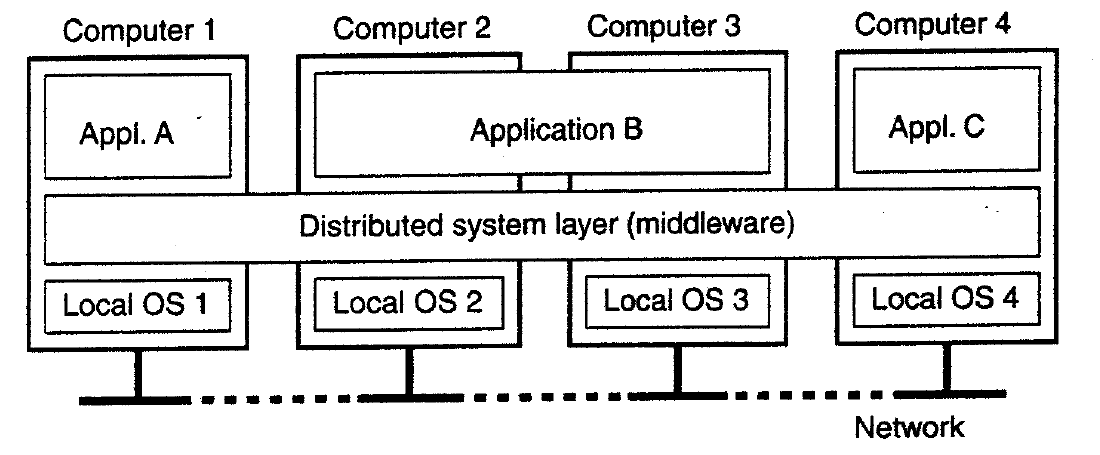
\includegraphics[width=\textwidth,keepaspectratio]{TanenbaumDistributed}
		\caption{A Distributed System visualised as \gls{middleware} \cite{tanenbaumdist}} 
		\label{fig:middleware}
	\end{figure}
\end{center}

\section{Blockchain}
Nofer et al. define \gls{blockchain}s as \say{data sets which are composed of a chain of data packages (blocks) where a block comprises multiple transactions. The \gls{blockchain} is extended by each additional block and hence represents a complete \gls{ledger} of the transaction history.} \cite{blockchain}. Nofer et al. describe the basic fundamentals of a \gls{blockchain}, which is that numerous blocks of transactions contribute to a larger chain. This chain is never controlled by a single body, instead a copy of the chain is stored at each node within a system, making \gls{blockchain} a popular candidate for controlling transactions over a decentralised computer system. Hence, \gls{blockchain} is the foundation for the vast majority of cryptocurrencies including Bitcoin\cite{bitcoin} and Ethereum\cite{ethereum}. One of the key aspects of \gls{blockchain} is the use of cryptographic \gls{hashing} algorithms, these algorithms represent a block as a fixed-length string. For a block to be added to the chain, it must contain the hash of the previous block.

\begin{center}
	\begin{figure}[H]
		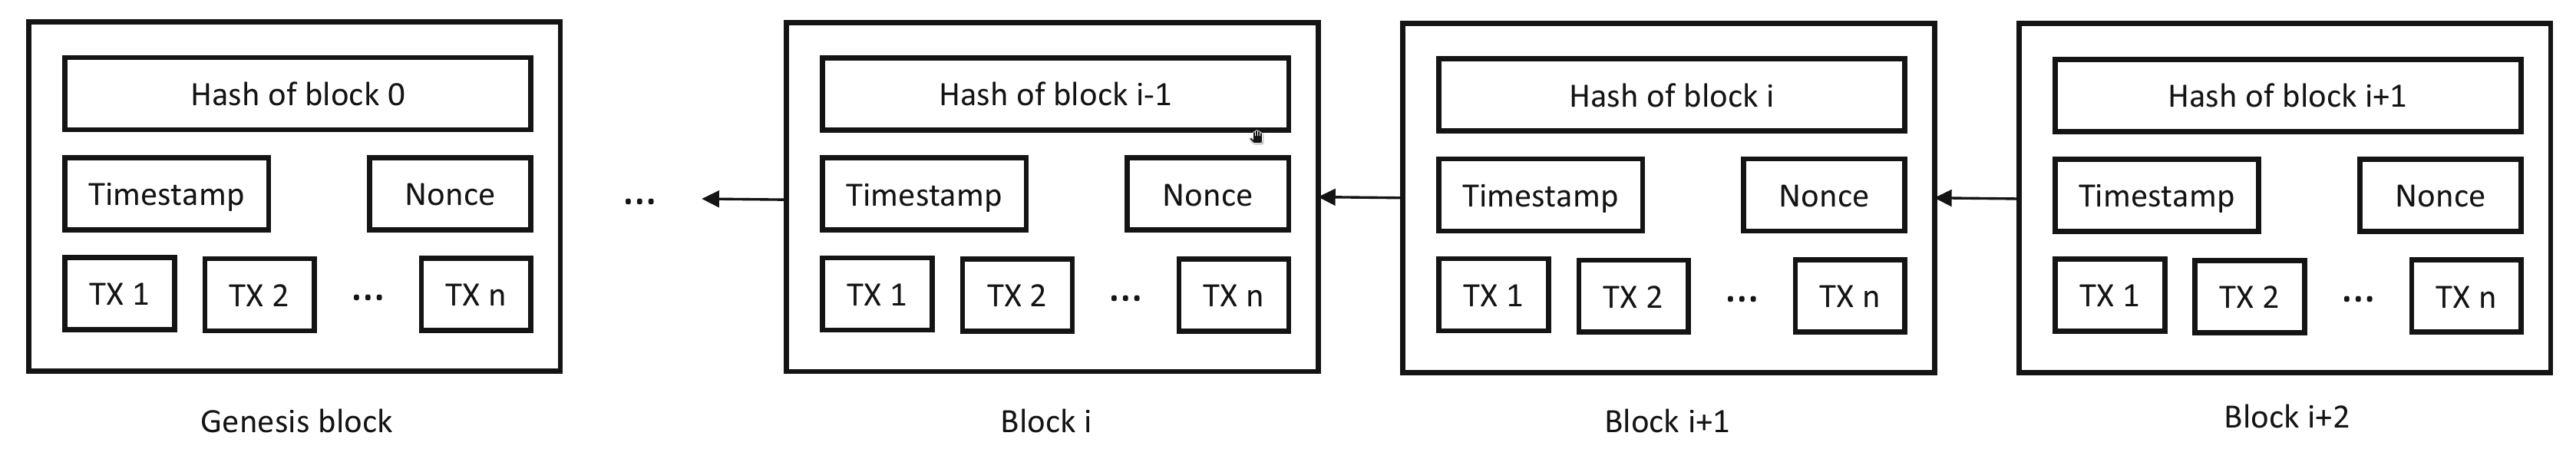
\includegraphics[width=\textwidth,keepaspectratio]{NoferBlock}
		\caption{An example of a \gls{blockchain} \cite{blockchain}} 
		\label{fig:blockchain}
	\end{figure}
\end{center}

%%%%%%%%%%%%%%%%%%
% AIMS AND OBJECTIVES
%%%%%%%%%%%%%%%%%%
\chapter{Project Aims and Objectives}

\section{Aim} \label{aim}
The original aim for this project was to design and create a decentralised firewall that could communicate knowledge of cyberattacks aimed at universities in real-time, allowing other universities to protect themselves from the same attacks. This system would be distributed, and hence must conform to the previous description of a distributed system in section \ref{distributed}. Following an extensive amount of background reading, there appeared to be no existing implementation or design of such a system which inspired me to alter my aim and instead focus entirely on designing a protocol and implementing a \gls{stub} to demonstrate the protocol's effectiveness. This project will therefore not be implementing a firewall, but instead a system to coordinate firewalls. Further research determined that \gls{blockchain} was the best choice for the underlying structure for such a protocol, and so this final change shaped the current aim for this project: \textbf{Using Blockchain to Create a Decentralised Security Model for Distributed Systems}.

\section{Objectives}
The following objectives provide an outline for what this project hopes to achieve:

\begin{enumerate}
    \item Evaluate the effectiveness of existing distributed security mechanisms.
    \item Investigate methods of establishing connections and synchronising computers within distributed systems.
    \item Understand the structure of \gls{blockchain}s and adapt them for firewall transactions.
    \item Implement and rest relevant resilience, fault tolerance and security mechanisms.
    \item Compare the use of decentralised security mechanisms.
\end{enumerate}

%%%%%%%%%%%%%%%%%%
% BACKGROUND
%%%%%%%%%%%%%%%%%%
\chapter{Background}

\section{Distributed Systems} \label{dist}
The primary reference used for distributed systems was Tanenbaum and van Steen's \say{Distributed Systems: Principles and Paradigms}\cite{tanenbaumdist}, who's literature provides an in-depth explanation from the fundamental theory of distributed systems to the design and implementation of such systems. Key details that were taken from this publication are detailed below. In general, this book covered the essential components of creating a distributed system, however much of the detail with regards to client-server interactions was not applicable to this project due to it's decentralised nature. Furthermore, a large portion of the book was not of interest to this project as it focuses on distributed processing, which only comprises a small element of this project, hence a large volume of information regarding implementation of processing was not useful.

\subsection{Architecture}
Tanenbaum and van Steen cover many aspects of a distributed system's architecture spanning network, software and physical architecture. This project will implement a decentralised, peer-to-peer network architecture, which will be discussed in detail in section \ref{decentrailsed}. The software used will consist primary of \gls{stub}s, which are used to hide the differences in machine architecture and communication between the computer and the distributed system. The combined use of \gls{stub}s creates a new software layer, known as \gls{middleware} which provides a common interface between a client application, and the distributed system. Creating this layer enables applications to communicate via an application-level protocol, which is independent from the protocol spoken by the \gls{middleware}.

\begin{figure}[H]
\centering
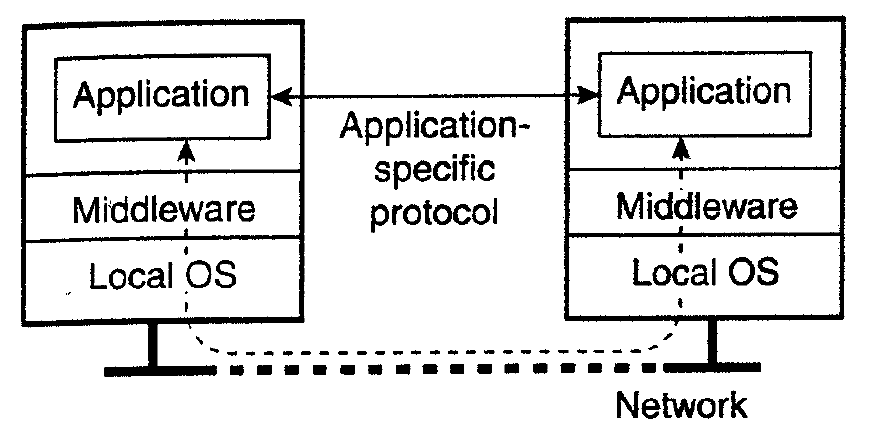
\includegraphics[height=5cm,keepaspectratio]{appl_layer_proto}
\caption{Application layer protocol running over \gls{middleware} \cite{tanenbaumdist}} 
\label{fig:middlewarelayers}
\end{figure}

With regards to physical architecture, Tanenbaum and van Steen discuss a number of approaches to client-server architectures, however due to the decentralised nature of this project, non of Tanenbaum and van Steen's classifications apply. 

\subsection{Remote Procedure Calls (RPC)}
Tanenbaum and van Steen introduce the concept of a \acrfull{RPC}. \acrshort{RPC}s are used to execute some action on a remote node within a distributed system.  Tanenbaum and van Steen provide a concise breakdown of the steps required to execute an \acrshort{RPC}:

\begin{enumerate}
    \item The client procedure calls the client \gls{stub} in the normal way.
    \item The client \gls{stub} builds a message and calls the local \acrfull{OS}.
    \item The client \acrshort{OS} sends the message to the remote \acrshort{OS}.
    \item The remote \acrshort{OS} gives the message to the server \gls{stub}.
    \item The server \gls{stub} unpacks the parameters and calls the server.
    \item The server does the work and returns the result to the \gls{stub}.
    \item The server \gls{stub} packs it in a message and calls it's local \acrshort{OS}.
    \item The server's \acrshort{OS} send the message to the client's acrshort{OS}.
    \item The client's \acrshort{OS} sends the message to the client \gls{stub}.
    \item The \gls{stub} unpacks the result and returns to the client.
\end{enumerate}

\begin{figure}[H]
\centering
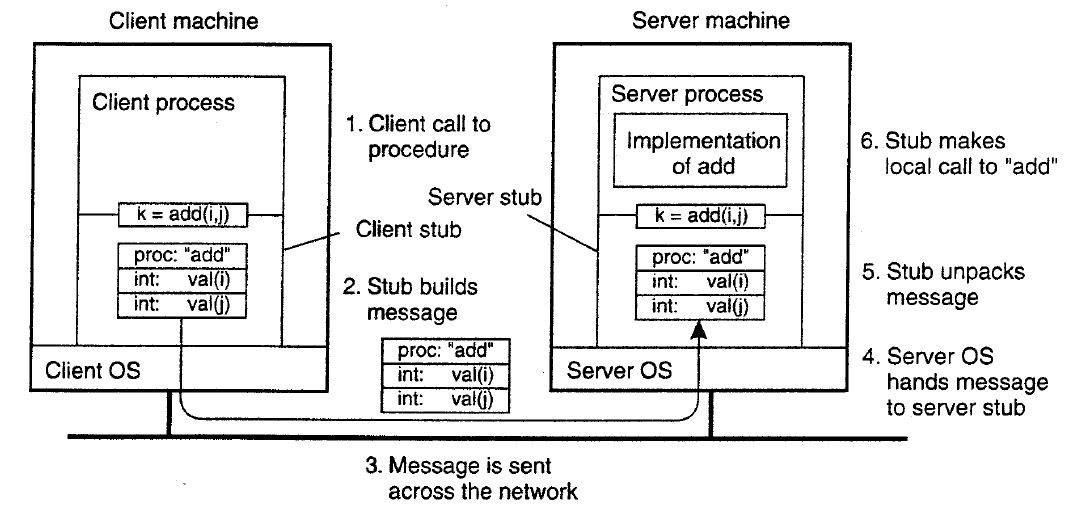
\includegraphics[width=\textwidth,keepaspectratio]{rpc}
\caption{A breakdown of an \acrshort{RPC} \cite{tanenbaumdist}} 
\label{fig:rpc}
\end{figure}

\section{Decentralised Systems} \label{decentrailsed}
Gray's \say{An Approach to Decentralized Computer Systems} \cite{decentralised} provided the basis for the decentralisation aspect of this project. Gray summarises the advantages of using decentralised systems, a number of which support the argument for using a decentralised topology in this project. The advantages which are relevant to this project are documented below.

\begin{itemize}
    \item \textbf{Capacity}: A decentralised system can support a large number of devices.
    \item \textbf{Response Time}: Having devices in close proximity can reduce response times.
    \item \textbf{Availability}: A failure is likely to be limited to a single site, allowing the rest of the system to continue normal operation.
    \item \textbf{Security}: Removing the central controller in a traditional distributed system removes the risk of an attack compromising the whole system.
\end{itemize}

Gray's article also looks at how decentralised systems should be designed including data types, network protocols and transactions. There are a number of similarities between Tanenbaum and van Steen's \acrshort{RPC}s and the structure Gray proposes for decentralised transactions. For this project however, the finer details proposed by Gray's system are not relevant as the literature uses a large number of examples base heavily on financial transactions, which contain a number of additional complexities over the transactions used within this project.


\section{Blockchain}
The primary reference used for \gls{blockchain} was Nofer et al.'s \say{Blockchain}\cite{blockchain}. Nofer et al. provide a high level overview of \gls{blockchain}, focusing primarily on the structure and implementation, with some consideration of the current applications of \gls{blockchain} in both financial and non-financial settings. Although concise, this publication provides a valuable summary of the essential components of blocks in order to create a ledger which can accurately trace transactions. Although not essential for this project, Nofer et al. additionally discuss how \gls{blockchain} can be implemented into smart contracts. In general, this literature was useful in providing a baseline for the structure of blocks within a \gls{blockchain}, and clearly explained the purpose of each field within the block, which allowed informed decisions to be made in regard to the structure of blocks used in this project. 

\begin{center}
	\begin{figure}[H]
		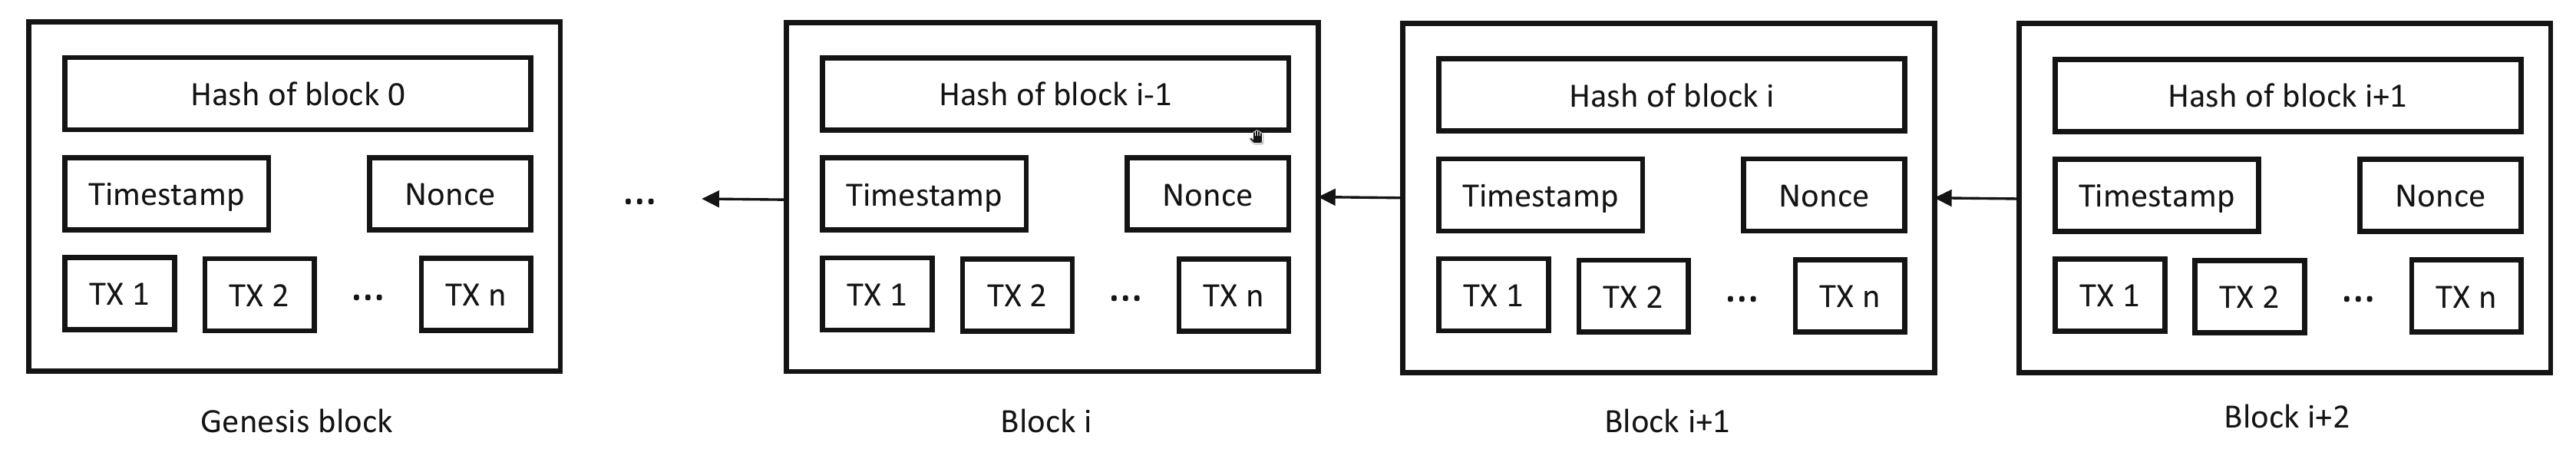
\includegraphics[width=\textwidth,keepaspectratio]{NoferBlock}
		\caption{An example of a \gls{blockchain} \cite{blockchain}} 
		\label{fig:blockchain2}
	\end{figure}
\end{center}

\section{Distributed Security}
The primary reference used for distributed security was Rivets and Lampson's \say{SDSI - A Simple Distributed Security Infrastructure} \cite{sdsi}. This publication provides an in-depth explanation of how a public-key infrastructure can be used in conjunction with access control lists to create a distributed security infrastructure. The majority of the literature within this publication is focussed on creating and issuing certificates, something that is not relevant for this project, however Rivets and Lampson did provide clear requirements over the data structures within such a system. Rivets and Lampson implement a message system similar to that of Tanenbaum and van Steen's in section \ref{dist}. The message system proposed by Rivets and Lampson contains only a type and dictionary of attributes.

\begin{figure}[H]
\centering
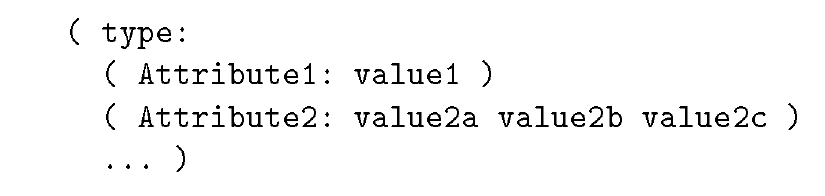
\includegraphics[height=2cm,keepaspectratio]{distmsg}
\caption{Message format for the SDSI Model \cite{sdsi}} 
\label{fig:sdsimessage}
\end{figure}

Additionally, Rivets and Lampson detail the concept of objects, which are defined by a type. This type is expressed in the form 

\begin{center} 
\texttt{protocol-name.message-type}
\end{center}

\section{Firewalls and Firewall Rules}
Al-Shaer and Hazem provide a detailed explanation of how firewall policies should be modelled and managed in \say{Modeling and Management of Firewall Policies} \cite{firewall}. This article explores methods of modelling policies and rules and provides a deep analysis of how those rules are interpreted by a firewall. The most relevant discussion within this literature is the structure of a firewall policy which is defined by Al-Shaer and Hazem as a set of rules, which act as records, with the following seven fields:

\begin{itemize}
    \item \textbf{Order}: The priority of a rule.
    \item \textbf{Protocol}: Either \acrfull{TCP} or \acrfull{UDP}.
    \item \textbf{Source IP}: The source IP address.
    \item \textbf{Source Port}: The source port.
    \item \textbf{Destination IP}: The destination IP address.
    \item \textbf{Destination Port}: The destination port.
    \item \textbf{Action}: The action the firewall should take (e.g. ACCEPT, DENY).
\end{itemize}

In regards to this project, there was little other relevant content in the literature. Following the change in this project's aim detailed in section \ref{aim}, this project was no longer concerned with the implementation of a firewall or the interpretation of firewall rules, which deemed the vast majority of Al-Shaer and Hazem's publication irrelevant.

Additional background information with regards to how firewalls are integrated into infrastructure came from Dulaney and Eastton's \say{CompTIA Security+ Study Guide: Exam SY0-501} \cite{comptiaSec}. Dulaney and Eastton's study guide covers a large number of aspects associated with cyber security, including technological, physical and psychological mitigations. With regards to firewalls, this publication details how the placement of firewalls can be used to form a \acrfull{DMZ}, which is a common network layout used by universities, as it permits certain areas of the network to be accessible from outside the local network.

\begin{figure}[H]
\centering
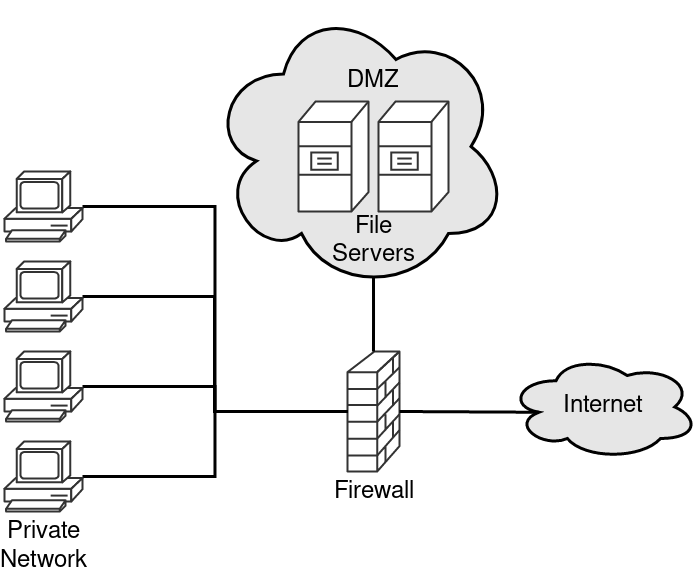
\includegraphics[height=10cm,keepaspectratio]{DMZ}
\caption{Using a firewall to create a \acrshort{DMZ}}
\label{fig:dmz}
\end{figure}

This information provided a strong understanding into where this project would fit in a standard network model. This publication also covered firewalls, however the information provided was not as detailed as that from Al-Shaer and Hazem, and hence no other aspects of this book were used.

\section{Fault Tolerance}
The primary reference for fault tolerance was Guerraoui and Schiper's \say{Fault-Tolerance by Replication in Distributed Systems}\cite{faulttol}. This literature details how replication can be used to provide fault tolerance in a distributed system in addition to ensuring consistency is maintained.  A number of backup techniques are discussed however the technique that is best suited for application is primary backup replication. Primary backup replication consists of a client invoking an operation which is the applied to the primary data, and then cascaded to a number of additional backups.

\begin{figure}[H]
\centering
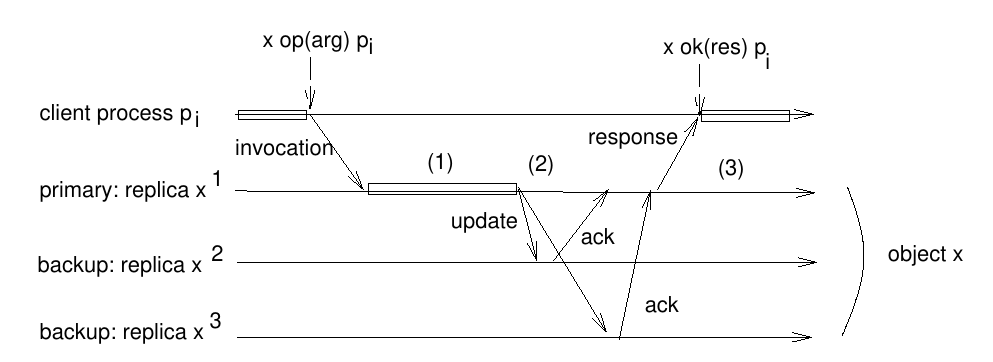
\includegraphics[height=5cm,keepaspectratio]{primback}
\caption{Primary backup technique \cite{faulttol}} 
\label{fig:backup}
\end{figure}

Guerraoui and Schiper continue to discuss methods of detecting faults and appropriate ways to deal with them. The methods covered however require a much greater level of control than that achievable by a single application running on a standard \acrshort{OS}, and hence are not applicable to this project.

\section{Computer Networks}
The primary reference for computer networks was Lammle's book \say{CompTIA Network+ Study Guide: Exam N10-007} \cite{comptiaNet}. Lammle's study guide covers a wide range of aspects associated with computer networks including physical implementations, subnets, security and protocols. Two sections which are relevant to this project are network layer protocols (\acrshort{TCP} and \acrshort{UDP}), and network topologies. Lammle provides a comprehensive explanation of the differences between \acrfull{TCP} and \acrfull{UDP}, however the difference that is most relevant to this project is \acrshort{TCP}'s requirement for a connection to be established prior to transmission. The book explains how establishing a \acrshort{TCP} connection takes additional time and blocks the port whilst attempting to establish a connection, which prevents any other connection from being made from that port. This is not ideal for a decentralised system as messages will be sent on an ad-hoc basis, with strict time constraints, and therefore \acrshort{UDP} will be more suitable for this project.

With regards to network topologies, Lammle details seven approaches: bus, star, ring, mesh, point-to-point, point-to-multipoint and hybrid. In order to create a truly decentralised distributed system, the mesh topology is best suited to this project. In a mesh topology, each device is connected to every other device, which provides the highest level of redundancy possible, as if one device were to crash, or a cable be disconnected, communication can continue via the other devices.

\begin{figure}[H]
\centering
\includegraphics[height=5cm,keepaspectratio]{mesh}
\caption{Mesh Topology} 
\label{fig:mesh}
\end{figure}

\section{Inter-Process Communication (IPC)}
Tanenbaum and Woodhull provide an extremely detailed breakdown of their UNIX based operating system in \say{Operating systems: Design and Implementation} \cite{operatingsystems}. This book covers all aspects of an \acrshort{OS}, providing insightful explanations of the decisions made at every step in the design process. As this project is designed to run as an application, many of the details covered in this publication are irrelevant, however Tanenbaum and Woodhull cover one essential aspect of this project: \acrfull{IPC}. \acrshort{IPC} is a function within many \acrlong{OS}s which enables multiple processes to communicate by passing messages to each other. \acrshort{IPC} will be the technique used to interact with the distributed system, as a client process will use \acrshort{IPC} to issue commands to the \gls{stub}. 

\chapter{Design}

\section{System Architecture}
The system will be compiled into one single executable binary, but will interface with a number of external libraries and the \acrshort{OS} via system calls. The stub will primarily communicate with the \acrshort{OS} in order to establish sockets and bind them to the desired ports, the framework will then communicate with the \acrfull{NIC} to obtain it's assigned \acrfull{IP} address. Whenever a new block is created or received, OpenSSL's libcrypto library \cite{libcrypto} will be used to generate or validate the block's hash. This interaction is visualised in the following component diagram.

\begin{figure}[H]
\centering
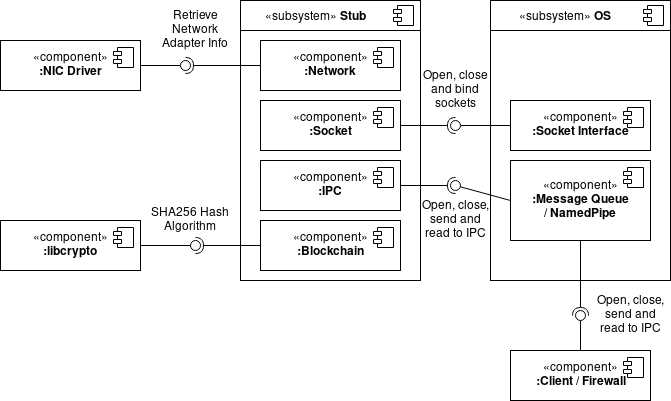
\includegraphics[height=8cm,keepaspectratio]{componentdiagram}
\caption{System Component Diagram} 
\label{fig:comp}
\end{figure}

\section{Data Structures}
The system uses two primary structures for storing data within the system, these are used for storing firewall rules and blocks.

\subsection{Firewall Rule} \label{rule}
The system supports five different actions that can be applied to a firewall rule: allow, deny, bypass, force allow and log.  These actions are supported by the distributed system but firewall software remains free to interpret these actions freely, which ensures consistency can be achieved despite different firewall vendors.
The firewall rule structure comprises of the following:

\begin{table}[H]
\centering
\begin{tabular}{ |c|c|c|c| } 
\hline
Field Name & Data Type & Size (Bytes) \\
\hline
source_addr & Character Array & 15 \\
source_port & Unsigned Integer & 2 \\
dest_addr & Character Array & 15 \\
dest_port & Unsigned Integer & 2 \\
action & FirewallAction & 1 \\
\hline
\end{tabular}
\caption{The Structure of a Firewall Rule}
\label{tab:rulestr}
\end{table}

This structure supports the standard model for firewall policies, supporting categorisation by the source address, source port, destination address and destination port. Each rule is then given an associated action.

\subsection{Firewall Block} \label{firewallblock}
Firewall blocks are used to create the chain of firewall rules within the system. These are comprised of the following fields:

\begin{table}[H]
\centering
\begin{tabular}{ |c|c|c|c| } 
\hline
Field Name & Data Type & Size (Bytes) \\
\hline
last_hash & Unsigned Char Array & Dependent on Hash Algorithm \\ 
author & Character Array & 15 \\
rule & FirewallRule & Dependent on machine architecture \\
next & FirewallBlock Pointer & Dependent on machine architecture \\
\hline
\end{tabular}
\caption{The Structure of a Firewall Block}
\label{tab:firewallblock}
\end{table}

The structure holds the last block hash in order to verify that the block has been validated and fits onto the chain. In addition to the last block hash, the structure includes the author of the block, which enables an audit to verify that the block was submitted by a reputable source. The structure contains a firewall rule which has been described previously in section \ref{rule}. Finally, the structure contains a pointer to another block, this field is used to join the blocks into a chain via a linked list. When a block is appended to the chain, this field will be null, however once the next block is added to the chain, this field will point to the new block.

\section{Message Structures}
The system uses two different message passing mechanisms, these being via the network for distributed transactions, and via \acrshort{IPC} for client - stub communication. Each message type follows a particular structure which is discussed below.

\subsection{Network} \label{netstruct}
For communications within the distributed system, three different message types are used: advertisement, consensus and rule. Furthermore, each message contains a subtype which is either a broadcast or an acknowledgement. All message types contain a set of common fields, which are detailed below.

\begin{table}[H]
\centering
\begin{tabular}{ |c|c|c|c| } 
\hline
Field Name & Data Type & Size (Bytes) \\
\hline
type & MessageType & 1 \\ 
subtype & MessageSubType & 1 \\ 
hops & Unsigned Integer & 1 \\ 
source_addr & Character Array & 15 \\
target_addr & Character Array & 15 \\
next_addr & Character Array & 15 \\
\hline
\end{tabular}
\caption{Common Fields in all Network Messages}
\label{tab:common}
\end{table}

The type field holds an enum which is called MessageType and contains three values: advertisement, consensus and rule. Similarly the subtype field holds an enum that contains two values: broadcast and acknowledgement. Broadcast messages are used to advertise a new device, request consensus and distribute new a firewall transaction, whereas acknowledgements are used to provide a response, such as acknowledging the new device and providing consensus for a proposed transaction. As the system is decentralised, messages are not sent directly to remote hosts as there may be devices on the network that another device is unaware of, which would result in unsynchronised \gls{blockchain}s. The use of a hop count allows us to limit the number of times a message can be sent around the network, essential to prevent older messages from clogging up the system. The last three fields contain addresses of devices. It may appear unnecessary to provide these values as the messages are wrapped in an \acrshort{IP} packet which already contains these values. These are necessary as when messages are relayed, the \acrshort{IP} packet contains the address of the most recent sender, overwriting the original information. The source address contains the address of the origin device, the target address contains the address of the final destination, and the next address contains the address of the next device to propagate the message to.

\subsubsection{Advertisement Messages}
The advertisement message is used to advertise the presence of a new device within the distributed system. This message contains no additional fields than those described in table \ref{tab:common}. When the advertisement message subtype is broadcast, the source address is set to the new device's \acrshort{IP} address. At least one host must be known to advertise on the network, and this host's address will be placed into the next address field. The target address field is not used for broadcasts as we have no specific target that we wish to send our message to. Once a node receives an advertisement broadcast, it will check whether that host is already known, if so, the message is ignored, and propagated, otherwise if the host is not yet known, the node first adds the new device to its list of known hosts, and then propagates the message. When the acknowledgement is sent, the target address is set to the address of the new device, which ensures that any other nodes which may have advertised do not interpret the acknowledgement as regarding their broadcast. Once the acknowledgement arrives at the new device, the node adds the host which sent the ack, but does not propagate the message.

\subsubsection{Consensus Messages}
The consensus message is used when a client or firewall submits a new firewall rule to the \gls{stub} via \acrshort{IPC}. This message contains one additional field which holds the hash of the last block. When a node proposes a new firewall rule, it must first submit the hash of it's last block, which is sent to all known hosts. On receipt of a consensus broadcast, the node calculates the hash of the last block on it's chain, and if it matches the hash sent in the message it sends an ack, and appends the origin node's address to a list of pending rules. The node then forwards the message to all known hosts. After broadcasting the message, the origin host resets a counter, which is incremented every time it receives an ack from one of it's known hosts. If this counter reaches atleast half of it's known hosts in some bounded time, it is deemed to have obtained consensus and may now distributed the new firewall rule.

\begin{table}[H]
\centering
\begin{tabular}{ |c|c|c|c| } 
\hline
Field Name & Data Type & Size (Bytes) \\
\hline
last_block_hash & Unsigned Char Array & Dependent on Hash Algorithm \\ 
\hline
\end{tabular}
\caption{Additional Fields in a Consensus Message}
\label{tab:consensus}
\end{table}

\subsubsection{Rule Messages}
The rule message is used to distribute a new firewall rule once a node has achieved consensus. Only the broadcast subtype is used for rule messages, as waiting for acknowledgements could halt the system at the time of an attack, which would prevent the node from responding to other attacks. Upon receiving a rule broadcast the node will check to see if has previously approved the transaction by looking up the rule's origin in its list of pending rules. If the origin exists in the pending rules then the new block will be added to the chain, including its author and the last hash, then propagated to all of the node's known hosts.

\begin{table}[H]
\centering
\begin{tabular}{ |c|c|c|c| } 
\hline
Field Name & Data Type & Size (Bytes) \\
\hline
rule & FirewallRule & Dependent on machine architecture \\ 
\hline
\end{tabular}
\caption{Additional Fields in a Rule Message}
\label{tab:rule}
\end{table}

\subsection{IPC}
There are four different types of \acrshort{IPC} message: rule, enable, disable, shutdown. The rule type is intended to be sent by a firewall, and contains a new firewall rule to be submitted to the distributed system. The enable and disable message types simply control the status of the stub, if it is believed that a host on the network may be malfunctioning (i.e. a firewall is sending bogus rules), it can be disabled and then re-enabled once the fault is fixed. Finally the shutdown message is used to properly terminate the \gls{stub}. Upon receiving the shutdown message, all sockets will be closed, the \acrshort{IPC} tunnel will be destroyed and the application will wait for all threads to terminate before exiting.
To ensure messages can be parsed correctly, all of these message types follow the same structure and simply do not use the redundant fields.

\begin{table}[H]
\centering
\begin{tabular}{ |c|c|c|c| } 
\hline
Field Name & Data Type & Size (Bytes) \\
\hline
message_type & IPCMessageType & 1 \\
rule & FirewallRule & Dependent on machine architecture \\
\hline
\end{tabular}
\caption{Structure of \acrshort{IPC} Messages}
\label{tab:ipc}
\end{table}
 
\section{ACR Protocol}
As described in section \ref{netstruct}, the system supports three message types: advertisement, consensus and rule, which form the ACR protocol.

\subsection{Advertisement}
The advertisement message is sent at startup and is mutually exclusive from the other messages, as it is executed automatically and does not affect the consensus or rule transaction stages. The advertisement message is sent when the framework is executed. The framework will send an advertisement broadcast to all known hosts, each of which will relay the message to each of their known hosts, provided that the hop count has not yet been exceeded. The known host will then forward the message to all of its known hosts, propagating the message throughout the network. Upon receiving an advertisement message, the host checks if the host is known, if not, it is added, and an acknowledgement is returned.

\begin{figure}[H]
\centering
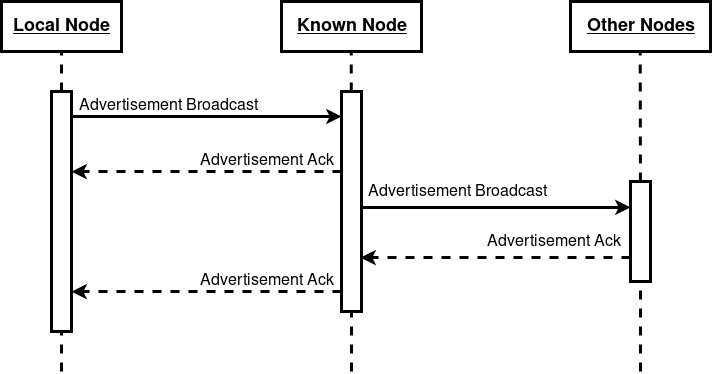
\includegraphics[width=\textwidth,keepaspectratio]{advertisement_seq}
\caption{Advertisement Sequence Diagram} 
\label{fig:advseq}
\end{figure}

\subsection{Consensus-Rule}
The consensus and rule messages are sent when a client or firewall send an \acrshort{IPC} message to the local \gls{stub}. Upon receiving the rule, the \gls{stub} will marshal the parameters into a network message, which is then sent to all known hosts. When a node receives the consensus message, it will compare the hash in the message to the hash of the previous block on its chain, if the hashes match, the block is considered valid and an acknowledgement is returned. The broadcast is then forwarded to all of the hosts known by that node. When the origin node receives an acknowledgement, it will check if that host is known. If it is not, then it will not increment the ack count, as it would interfere with the consensus calculation, however it will still receive the rule, if consensus is achieved. The origin node will then wait for some timeout, after which it will test if a sufficient number of acknowledgements have been received in comparison to the number of known hosts. If this test passes (e.g. at least half of the known hosts must acknowledge), then a rule message is sent. No acknowledgements are sent upon receipt of a rule message, but nodes will continue to propagate the message until the hop limit is reached.

\begin{figure}[H]
\centering
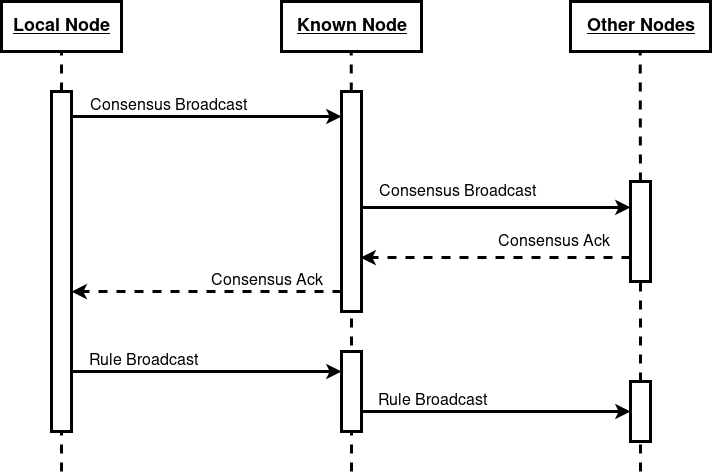
\includegraphics[width=\textwidth,keepaspectratio]{consensus_rule_seq}
\caption{Successful Consensus-Rule Sequence Diagram} 
\label{fig:consruleseq}
\end{figure}

\chapter{Implementation}

\section{Language}
The logic within this project could be achieved using a range of programming languages, however such a system needs to be reliable and fast, which narrows down the applicable languages. As cross compatibility is desirable, Java\cite{java} or Python\cite{python} may seem like the best options as Java executes entirely within the Java Virtual Machine (JVM)\cite{jvm} and Python is executed using an interpreter. Each of these technologies provide a suitable abstraction such that if the \acrshort{VM} or interpreter is supported by an \acrshort{OS}, it should work. The drawbacks associated with this are that a \acrshort{VM} or interpreter introduce a large memory overhead, something that is not desirable given this framework is intended to be implemented into edge devices, additionally, with such abstractions we lose both speed and control. Rust\cite{rust} is a modern language focused on performance and reliability, however its immaturity leaves a number of features missing or poorly implemented as it currently relies heavily on community submitted modules. One advantage of Rust however is its low memory footprint, and memory management, which enables small binary executables to be built, ideal for this project. 

The final two languages considered were C\cite{c} and C++\cite{cpp}. It may seem an obvious choice to use C++ over C, however for this project very few features of C++ would be useful, and would simply add additional steps in the program to bridge between \acrfull{POSIX} functions (implemented in C) and C++ types and syntax. One advantage that C has over C++ is its existing dominance in operating systems. Deemed the \textit{system programming language}, the Linux\cite{linux} and NetBSD\cite{netbsd} kernels are written in pure C, along with the vast majority of the FreeBSD\cite{freebsd} and Windows\cite{windows} kernels. This means that using C enables this project to be compiled into an operating system, such that the distributed system is automatically instantiated on boot in kernel space and cannot be stopped or interrupted by a malicious application or user. Furthermore, writing this project in C allows wrappers to be written for all other languages, C++ can be integrated with no changes, and modules can be written for most other languages including Java and Python.

\section{IPC}
In order to achieve cross-platform \acrshort{IPC}, different approaches were required for \acrfull{POSIX} compliant operating systems and Windows\cite{windows} operating systems. Each \acrshort{OS} type offers a number of \acrshort{IPC} methods, which are briefly discussed the following sections.

The \gls{stub} provides the following abstractions for interfacing with native \acrshort{IPC}. The implementation methods are discussed in their relative sections below.\\\\

\begin{lstlisting}[language=c,style=c,caption=IPC API]
int init_ipc_server(void);
int init_ipc_client(void);
int connect_ipc(void);
int cleanup_ipc(void);
int send_ipc_message(IPCMessage *message);
int recv_ipc_message(IPCMessage *message);
\end{lstlisting}

\subsection{POSIX} \label{posixipc}
\acrshort{POSIX} systems provide four interfaces for \acrshort{IPC}: pipes, FIFO, message queues and sockets. Although pipes do allow processes to communicate, the primary purpose of pipes is to obtain the output of one command and pass this output into a second command, which is not suitable for our application. FIFO and message queues operate very similarly, whereby each method creates some file in the filesystem which can then be referenced by any process. FIFO is the predecessor to message queues, and hence different operating systems have varying implementations for FIFO, however as message queues are a \acrshort{POSIX} standard, all implementations provide the same interface, greatly simplifying the processes of making this project cross compatible. For this reason, message queues were used for \acrshort{POSIX} \acrshort{IPC}. The final method is via UNIX sockets. The socket interface is primarily designed for networked communication, but also supports \acrshort{IPC}. Unfortunately, as sockets are intended for use in networks, some implementations still use the \acrshort{NIC} to communicate even locally, which slows down communication, and adds additional points of failure.

\begin{lstlisting}[language=c,style=c,caption=Creating the message queue on a POSIX OS]
mqueue = mq_open("/dfw", O_CREAT | O_RDWR, 0644, &attr);
\end{lstlisting}

Whilst testing this application it was discovered that nobody had yet created an interface for \acrshort{POSIX} message queues in Java, so a secondary project was created, called Jmq \cite{jmq} which provides an interface for \acrshort{POSIX} message queues in Java using the Java Native Interface (JNI). This enables a \gls{stub} to be created in Java by passing messages using the following syntax:\\

\begin{lstlisting}[language=java,style=java,caption=Example of Jmq]
Jmq_attr attrs = new Jmq_attr(0, 2, 1, 0);
Jmq my_queue = new Jmq("/dfw", Jmq.O_CREAT | Jmq.O_RDWR, 0644, attrs);
my_queue.unlink();
\end{lstlisting}

\subsection{Windows}
Windows\cite{windows} offers three methods of \acrshort{IPC}: Anonymous Pipes, Named Pipes and sockets. Anonymous pipes allow half-duplex communication, which is not ideal for this project, as it is necessary for the client / firewall to send instructions to the \gls{stub}, and for the \gls{stub} to send messages back to the client. Furthermore, Hart\cite{windowsprog} explains the fundamental issue with anonymous pipes: they have no identifier associated with them, which creates a new problem of communicating the pipe handle to any clients wishing to connect. Named pipes are full-duplex, message oriented pipes than can operate locally or over a network. The difference between anonymous and named pipes is that a named pipe can be identified using a string which represents a file path, this enables both client and \gls{stub} to connect directly to the pipe. The final method is via sockets which act similarly to UNIX sockets, and hence have the same pitfalls as UNIX sockets mentioned in section \ref{posixipc}.\\

\begin{lstlisting}[language=c,style=c,caption=Creating the message queue on Windows]
mqueue = CreateNamedPipe(TEXT("\\\\.\\pipe\\dfw"),
                           PIPE_ACCESS_DUPLEX | FILE_FLAG_OVERLAPPED,
                           PIPE_TYPE_MESSAGE, 1, 0, 0, 0, NULL);
\end{lstlisting}

\section{Sockets}
Network sockets are the primary method allowing processes to communicate over a network, however similarly to \acrshort{IPC}, \acrshort{POSIX} and Windows system provide slightly different socket interfaces. A numeric port is bound to the socket which enables the network stack to communicate with the socket, and hence the process. The main difference is that Windows requires the initialisation of the WinSock\cite{winsock} library. Thankfully other than the initialisation of WinSock, the rest of the interface provided by WinSock is very similar to the basis of \acrshort{POSIX} sockets, which are known as Berkeley sockets. This similarity means that only small modification need to be made to the source code. After creating the socket, it is then bound to the numeric port. The default ports used for this project are 8070 and 8071.

The \gls{stub} provides the following abstractions for interfacing with native sockets.
\begin{lstlisting}[language=c,style=c,caption=Socket API]
int init_sockets(void);
int cleanup_sockets(void);
socket_t create_socket(void);
void close_socket(socket_t sock);
int bind_socket(socket_t sock, int port);
int send_to_socket(socket_t sock, void *message, size_t length, int flags,
                   struct sockaddr_in dest_addr);
int recv_from_socket(socket_t sock, void *buffer, size_t length, int flags);
\end{lstlisting}

\section{Network}
As the project is focussed on creating a distributed system, the vast majority of the implementation is based on networking. Thankfully, due to the previous abstractions created regarding sockets, the network implementation consists primarily of the business logic. The one major difference between the UNIX network stack, and the Windows network stack, is querying the \acrshort{OS} to retrieve information from \acrshort{NIC}s. Implementing this required an entirely different system for each operating system. On UNIX, the \texttt{getifaddrs} function was used, whereas on Windows, the \texttt{GetAdaptersAddresses} function was used.

The \gls{stub} provides the following abstractions for interfacing with the native network stack.
\begin{lstlisting}[language=c,style=c,caption=Network API]
int get_local_address(char *buffer);
int get_acks(void);
int reset_acks(void);
int set_ack(char *addr);
int load_hosts_from_file(const char *fname);
int save_hosts_to_file(const char *fname);
int add_host(char* addr);
int check_host_exists(char *addr);
int get_host_count(void);
int init_net(void);
int cleanup_net(void);
int send_to_host(char *ip_address, void *message, size_t length);
int send_advertisement_message(AdvertisementMessage *message);
int send_to_all_advertisement_message(AdvertisementMessage *message);
int recv_advertisement_message(void *buffer);
int recv_advertisement_broadcast(AdvertisementMessage *message);
int recv_advertisement_ack(AdvertisementMessage *message);
int send_consensus_message(ConsensusMessage *message);
int send_to_all_consensus_message(ConsensusMessage *message);
int recv_consensus_message(void *buffer);
int recv_consensus_broadcast(ConsensusMessage *message);
int recv_consensus_ack(ConsensusMessage *message);
int send_rule_message(RuleMessage *message);
int send_to_all_rule_message(RuleMessage *message);
int recv_rule_message(void *buffer);
int recv_rule_broadcast(RuleMessage *message);
int poll_message(void *buffer, size_t length);
\end{lstlisting}

\section{Multithreading}
In order for the \gls{stub} to be capable of consecutively send and receive messages over both the network, and via \acrshort{IPC}, the framework had to be multithreaded. Unsurprisingly, \acrshort{POSIX} and Windows use different thread models, which means there is no common threading interface. Thankfully, the \acrshort{POSIX} thread model has been ported to Windows in the form of the \acrshort{POSIX} Threads for Windows project\cite{pthread}. This allows the source code to be written identically for all operating systems, the only difference being that Windows will be linked with the necessary Dynamic-Link Library (DLL).

\section{Blockchain}
Once the previous \acrshort{API}s had been created, the \gls{blockchain} aspect of the project could be implemented. As the structure of these blocks have already been discussed in section \ref{firewallblock}, this section will focus on how the functionality of this was implemented, primarily the hashing of blocks.

\subsection{Hash Algorithms} 
The first decision that had to be made was which hash algorithm to implement. A wide range of hash algorithms are available, however the most popular three are Secure Hash Algorithm (SHA), MD5 and BLAKE. The SHA hash suite boasts a number of algorithms which are classed into four generations: SHA-0, SHA-1, SHA-2 and SHA-3. The SHA-0 and SHA-1 algorithms are the least secure, and are now deemed insecure as collisions been found, which would enable a malicious block to contain the hash of a valid block. At the time of writing this, there are no known collisions for the SHA-2 or SHA-3 families. The MD5 hash algorithm is also insecure for the same reason as SHA-1 and is hence not appropriate for this project. The final algorithm family is BLAKE, which consists of three families: BLAKE, BLAKE2 and BLAKE3. There are no known collisions within any of the BLAKE hash families, however the BLAKE algorithm has not been tested for \gls{blockchain} applications, whereas the SHA family has. For this reason, this project will utilise the same hash algorithm as Bitcoin \cite{bitcoin}, SHA-256.

\begin{table}[H]
\centering
\begin{tabular}{ |c|c|c|c|c| } 
\hline
\multicolumn{2}{|c|}{Hash Algorithm} & Output Size & Collisions found? & Used By \\
\hline
\multicolumn{2}{|c|}{MD5} & 128 & Yes & None \\
\hline
\multicolumn{2}{|c|}{SHA-0} & 160 & Yes & None \\
\hline
\multicolumn{2}{|c|}{SHA-1} & 160 & Yes & None \\
\hline
\multirow{6}*{SHA-2} & SHA-224 & 224 & No & None \\
& SHA-256 & 256 & No & Bitcoin\cite{bitcoin}, Bitcoin Cash \\
& SHA-384 & 384 & No & None \\
& SHA-512 & 512 & No & None \\
& SHA-512/224 & 224 & No & None \\
& SHA-512/256 & 256 & No & None \\
\hline
\multirow{4}*{SHA-3} & SHA3-224 & 224 & No & None \\
& SHA3-256 & 256 & No & None \\
& SHA3-384 & 384 & No & None \\
& SHA3-512 & 512 & No & None \\
\hline
\multirow{4}*{BLAKE} & BLAKE-224 & 224 & No & None \\
& BLAKE-256 & 256 & No & None \\
& BLAKE-384 & 384 & No & None \\
& BLAKE-512 & 512 & No & None \\
\hline
\multirow{2}*{BLAKE2} & BLAKE2s & 256 & No & Nano\cite{nano} \\
& BLAKE2b & 512 & No & None \\
\hline
\multicolumn{2}{|c|}{BLAKE3} & Variable & No & None \\
\hline
\end{tabular}
\caption{Comparison of Hash Algorithms}
\label{tab:hashalgo}
\end{table}

\subsection{Hash Implementation}
When implementing the desired hash algorithm, there were to primary options, to implement the algorithm from scratch, or to use an existing library. If the algorithm was to be implemented from scratch, then the resulting application would requires less dependencies and would overall result in a more self-contained binary. Using a library would result in one additional dependency, however the vast number of algorithms provided by most libraries would allow the entire \gls{blockchain} and protocol to be easily updated should a more secure algorithm be preferable. Furthermore, most libraries are thoroughly tested and well engineered to guarantee the most efficient operation and make sure the algorithms can handle every edge case. For this it was decided that an external library would be implemented, and a breakdown of the considered libraries is provided below \cite{hashlibcomp}.

\begin{table}[H]
\centering
\begin{tabular}{ |c|c|c|c|c| } 
\hline
Cryptography Library & Algorithm Families & Language & Compatible OSs & First Created\\
\hline
OpenSSL (libcrypto)\cite{libcrypto} & 9 & C & 28 & 1998\\
wolfSSL (wolfCrypt)\cite{wolfCrypt} & 6 & C & 26 & 2006\\
cryptlib\cite{cryptlib} & 6 & C & 37 & 1995\\
GPG (Libgcrypt)\cite{libgcrypt} & 11 & C & Unknown & 1999\\
\hline
\end{tabular}
\caption{Comparison of Cryptographic Libraries}
\label{tab:cryptolib}
\end{table}

From the previous table, it is apparent that libgcrypt supports the most algorithms from the comparison given in \cite{hashlibcomp}, however for cross compatibility, cryptlib boasts 37 supported operating systems. OpenSSL's libcrypto sits in the middle of the two, supporting nine hash algorithm families and 28 different operating systems. Additionally, libcrypto is has been the default cryptography library distributed with most Linux, BSD and Windows operating systems, meaning it has received a large amount of support, and faced tight scrutiny by the likes of Microsoft. This made libcrypto the optimum library for use in this project. 

\section{Fault Tolerance}

\chapter{Testing}

\chapter{Evaluation}

\chapter{Conclusion}

\printglossaries

\bibliography{bib} 
\bibliographystyle{ieeetr}

\appendix

\iffalse
\chapter{Framework Source Code}
\lstinputlisting[language=c,style=c,caption=main.c,basicstyle=\ttfamily\scriptsize]{../src/main.c}
\lstinputlisting[language=c,style=c,caption=blockchain.h,basicstyle=\ttfamily\scriptsize]{../src/blockchain.h}
\lstinputlisting[language=c,style=c,caption=blockchain.c,basicstyle=\ttfamily\scriptsize]{../src/blockchain.c}
\lstinputlisting[language=c,style=c,caption=firewall.h,basicstyle=\ttfamily\scriptsize]{../src/firewall.h}
\lstinputlisting[language=c,style=c,caption=firewall.c,basicstyle=\ttfamily\scriptsize]{../src/firewall.c}
\lstinputlisting[language=c,style=c,caption=ipc.h,basicstyle=\ttfamily\scriptsize]{../src/ipc.h}
\lstinputlisting[language=c,style=c,caption=ipc.c,basicstyle=\ttfamily\scriptsize]{../src/ipc.c}
\lstinputlisting[language=c,style=c,caption=net.h,basicstyle=\ttfamily\scriptsize]{../src/net.h}
\lstinputlisting[language=c,style=c,caption=net.c,basicstyle=\ttfamily\scriptsize]{../src/net.c}
\lstinputlisting[language=c,style=c,caption=socket.h,basicstyle=\ttfamily\scriptsize]{../src/socket.h}
\lstinputlisting[language=c,style=c,caption=socket.c,basicstyle=\ttfamily\scriptsize]{../src/socket.c}

\chapter{Client Program Source Code}
\lstinputlisting[language=c,style=c,caption=client.c,basicstyle=\ttfamily\scriptsize]{"../src/example\string_client/client.c"}

\chapter{Code and Framework Documentation}
\includepdf[pages=-]{../docs/latex/refman.pdf}
\fi

\end{document}